\section{Security and User Privacy Vulnerabilities of Instant Messaging System}
\label{sec:security-and-user-privacy-vulnerabilities-of-instant-messaging-system}

\begin{figure}[H]
    \centering
    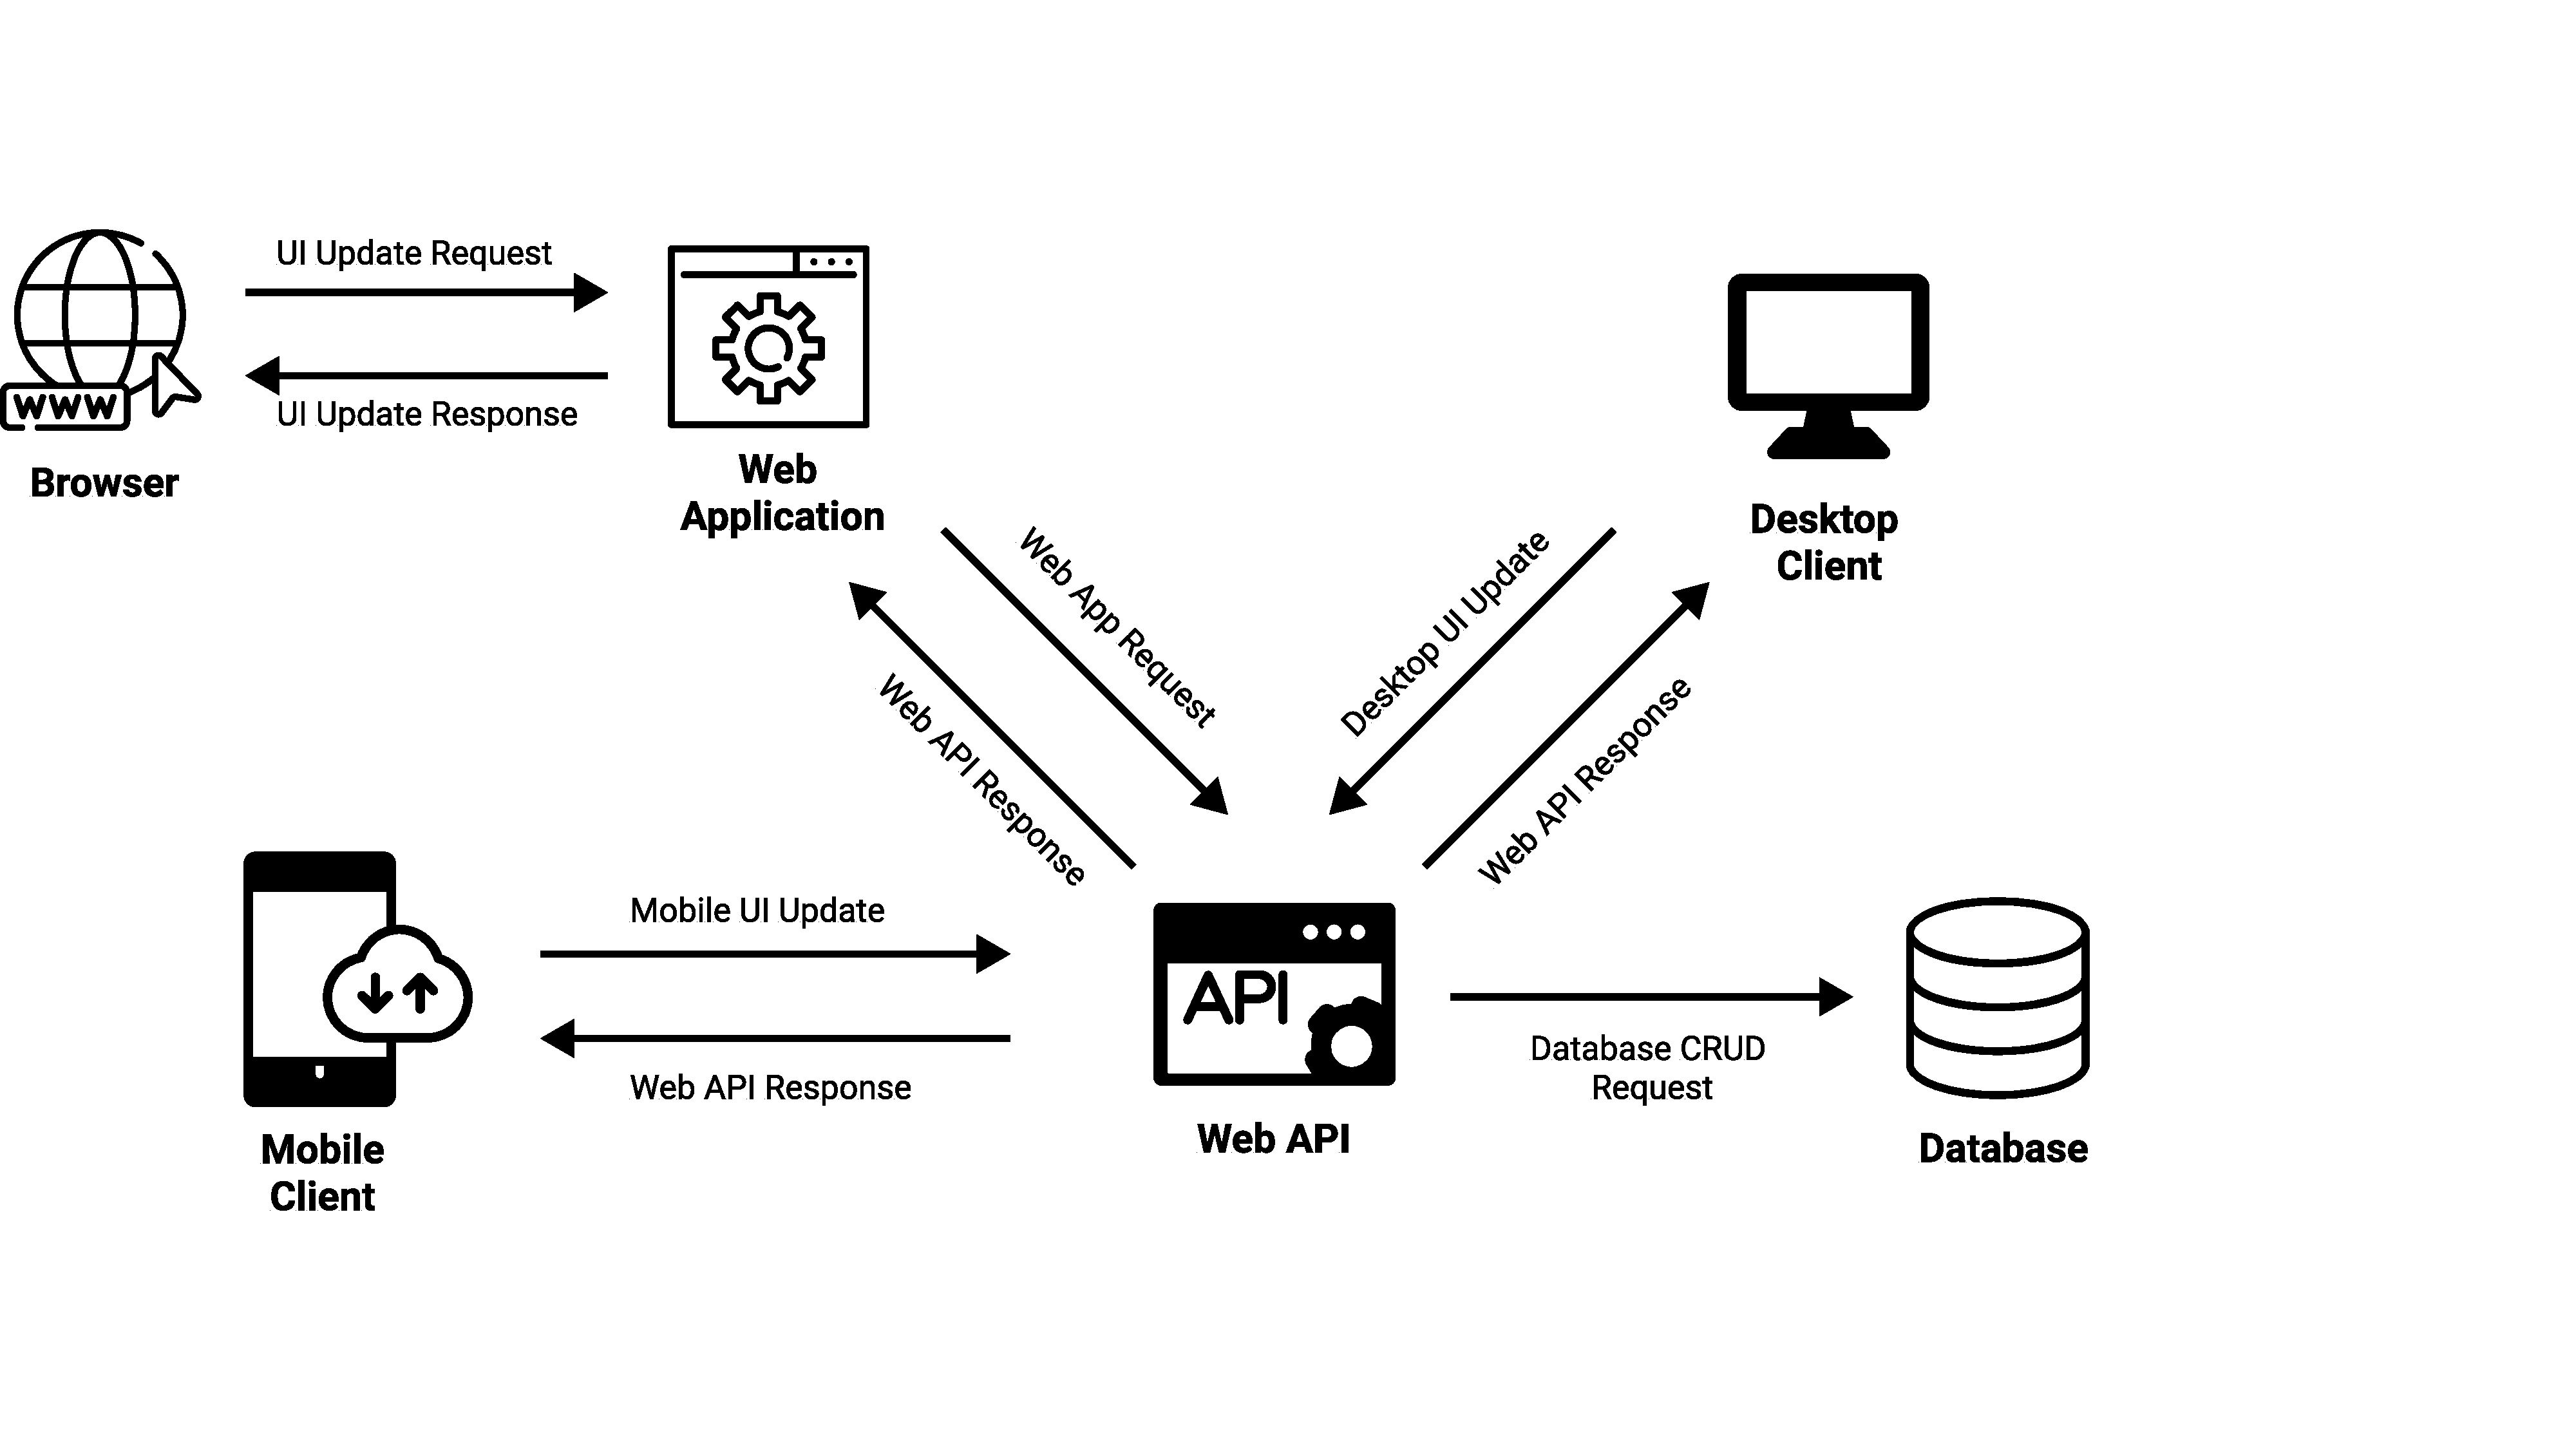
\includegraphics[width=1.2\textwidth]{Pictures/Threat_Modeling}
    \caption{Database diagram.}\label{fig:figure6}
\end{figure}

\begin{enumerate}
    \item \textbf{Browser UI Update Request}
    \begin{itemize}
        \item \textbf{Treat 1.1.} An adversary can perform action on behalf of other user due to lack of controls against cross domain requests.
        \item \textbf{Treat 1.2.} An adversary may bypass critical steps or perform actions on behalf of other users (victims) due to improper validation logic.
        \item \textbf{Treat 1.3.} An adversary can reverse weakly encrypted or hashed content.
        \item \textbf{Treat 1.4.} An adversary may gain access to sensitive data from log files.
        \item \textbf{Treat 1.5.} An adversary can spoof the target web application due to insecure TLS certificate configuration.
        \item \textbf{Treat 1.6.} An adversary can steal sensitive data like user credentials.
        \item \textbf{Treat 1.7.} An adversary can gain access to sensitive data stored in Web App's config files.
        \item \textbf{Treat 1.8.} An adversary can gain access to sensitive data by performing SQL injection through Web App.
        \item \textbf{Treat 1.9.} An attacker steals messages off the network and replays them in order to steal a user's session.
        \item \textbf{Treat 1.10.} An adversary can deface the target web application by injecting malicious code or uploading dangerous files.
        \item \textbf{Treat 1.11.} An adversary may spoof Desktop Web Browser (Chrome) and gain access to Web Application.
        \item \textbf{Treat 1.12.} An adversary can create a fake website and launch phishing attacks.
        \item \textbf{Treat 1.13.} Attackers can steal user session cookies due to insecure cookie attributes.
        \item \textbf{Treat 1.14.} An adversary can get access to a user's session due to insecure coding practices.
        \item \textbf{Treat 1.15.} An adversary can get access to a user's session due to improper logout and timeout.
        \item \textbf{Treat 1.16.} Attacker can deny the malicious act and remove the attack foot prints leading to repudiation issues.
        \item \textbf{Treat 1.17.} An adversary may gain access to sensitive data from uncleared browser cache.
        \item \textbf{Treat 1.18.} An adversary can gain access to sensitive information through error messages.
        \item \textbf{Treat 1.19.} An adversary can gain access to sensitive data by sniffing traffic to Web Application.
        \item \textbf{Treat 1.20.} An adversary can gain access to certain pages or the site as a whole.
        \item \textbf{Treat 1.21.} An adversary may gain access to unmasked sensitive data such as credit card numbers.
    \end{itemize}
    \item \textbf{Web App Request}
    \begin{itemize}
        \item \textbf{Treat 2.1.} An adversary may gain unauthorized access to Web API due to poor access control checks.
        \item \textbf{Treat 2.2.} An adversary can gain access to sensitive information from an API through error messages.
        \item \textbf{Treat 2.3.} An adversary can gain access to sensitive data by sniffing traffic to Web API\@.
        \item \textbf{Treat 2.4.} An adversary can gain access to sensitive data stored in Web API's config files.
        \item \textbf{Treat 2.5.} Attacker can deny a malicious act on an API leading to repudiation issues.
        \item \textbf{Treat 2.6.} An adversary may spoof Mango Web Application and gain access to Web API\@.
        \item \textbf{Treat 2.7.} An adversary may inject malicious inputs into an API and affect downstream processes.
        \item \textbf{Treat 2.8.} An adversary can gain access to sensitive data by performing SQL injection through Web API\@.
    \end{itemize}
    \item \textbf{Web API Response}
    \begin{itemize}
        \item \textbf{Treat 3.1.} An adversary can reverse weakly encrypted or hashed content.
        \item \textbf{Treat 3.2.} An adversary may gain access to sensitive data from log files.
        \item \textbf{Treat 3.3.} An adversary can gain access to sensitive information through error messages.
        \item \textbf{Treat 3.4.} Attacker can deny the malicious act and remove the attack foot prints leading to repudiation issues.
        \item \textbf{Treat 3.5.} An adversary can spoof the target web application due to insecure TLS certificate configuration.
        \item \textbf{Treat 3.6.} An adversary can steal sensitive data like user credentials.
        \item \textbf{Treat 3.7.} An adversary can create a fake website and launch phishing attacks.
    \end{itemize}
    \item \textbf{CRUD Request}
    \begin{itemize}
        \item \textbf{Treat 4.1.} An adversary can gain unauthorized access to database due to loose authorization rules.
        \item \textbf{Treat 4.2.} An adversary can gain access to sensitive PII or HBI data in database.
        \item \textbf{Treat 4.3.} An adversary can gain access to sensitive data by performing SQL injection.
        \item \textbf{Treat 4.4.} An adversary can deny actions on database due to lack of auditing.
        \item \textbf{Treat 4.5.} An adversary can tamper critical database securables and deny the action.
        \item \textbf{Treat 4.6.} An adversary may leverage the lack of monitoring systems and trigger anomalous traffic to database.
        \item \textbf{Treat 4.7.} An adversary can gain unauthorized access to database due to lack of network access protection.
    \end{itemize}
    \item \textbf{Mobile UI Update}
    \begin{itemize}
        \item \textbf{Treat 5.1.} An adversary can gain access to sensitive data by performing SQL injection through Web API.
        \item \textbf{Treat 5.2.} An adversary can reverse engineer and tamper binaries.
        \item \textbf{Treat 5.3.} An adversary may inject malicious inputs into an API and affect downstream processes.
        \item \textbf{Treat 5.4.} An adversary may spoof Mobile App (IOS, Android) and gain access to Web API\@.
        \item \textbf{Treat 5.5.} An adversary obtains refresh or access tokens from Mobile App (IOS, Android) and uses them to
        obtain access to the Mango Web API\@.
        \item \textbf{Treat 5.6.} Attacker can deny a malicious act on an API leading to repudiation issues.
        \item \textbf{Treat 5.7.} An adversary can gain access to sensitive data stored in Web API's config files.
        \item \textbf{Treat 5.8.} An adversary can gain sensitive data from mobile device.
        \item \textbf{Treat 5.9.} An adversary can gain access to sensitive data by sniffing traffic to Web API\@.
        \item \textbf{Treat 5.10.} An adversary can gain access to sensitive data by sniffing traffic from Mobile client.
        \item \textbf{Treat 5.11.} An adversary can gain access to sensitive information from an API through error messages.
        \item \textbf{Treat 5.12.} An adversary may gain unauthorized access to Web API due to poor access control checks.
        \item \textbf{Treat 5.13.} An adversary may jail break into a mobile device and gain elevated privilege.
    \end{itemize}
\end{enumerate}